\section{Quantum algorithms}

It's now to see some important quantum circuits that can be used in practice in order to obtain interesting results or behaviour inside a quantum computer. A lot of them will be not usefull per se, but are really important for the creation of larger and more powerful schemes.

\subsection{Quantum Fourier Transform}

The aim is to create an algorithm that bring the computational basis into the Fourier base, defined by the application of the Fourier transform on the vectors of the base itself. Therefore, we need first to recall the definition of discrete fourier transform which is given by.
\dfn{Discrete Fourier transform}
{
    Taken a vector $(x_1, x_2, \dots, x_N)\in \mathbb{C}^N$ it's Fourier transform is an application $\mathcal{U}: \mathbb{C}^N \to \mathbb{C}^N$ that actes in the following way
    \begin{align}
        &\mathcal{U}\vb{x} = \vb{y}, &y_k = \frac{1}{\sqrt{N}} \sum_{j=1}^N e^{i2\pi \frac{jk}{N}}x_j.
    \end{align} 
}
\noindent
We know that such an application posses a lot of properties, in particular we know how the following realtions are true
\begin{align}
    \label{eq:DiscrFourTrans}
    &\mathcal{U}^{-1} = \mathcal{U}^*, &\mathcal{U}^{-1} = \mathcal{U}^\dagger,
\end{align}
meanging that it's a particular unitary transformation, and so we imagine that a circuit can represent it.

We basically want to create an algorithm that allows us to take the computational basis and perform \eqref{eq:DiscrFourTrans} on it. In order to do that we will use a particular notation to describe the computational base of an $N$ qubit system, using the binary representation.
\dfn{Binary representation}
{
    Taken a system of $N$ qubit, where the computational base has the form $\{\ket{00\dots 0}, \ket{00\dots 1}, \dots\}$ we will write down the element s of the basis as $\{\ket{j}\}_{j=0}^{2^N-1}$ where the following relation is given
    \begin{align}
        &\ket{j} = \ket{j_1j_2\dots j_N}, &j = \sum_{i=1}^N j_i 2^{}.
    \end{align}
    basically $j$ is the number described by the system state in binary base.
}
\noindent
Using this notation it's really easy to write down the Fourier transform of the base having that
\begin{equation}
    \label{eq:QFT}
    \mathcal{U}\ket{j} = \frac{1}{2^{N/2}} \sum_{k=0}^{2^N-1} e^{i2\pi \frac{jk}{2^N}} \ket{k},
\end{equation}
having that the base is brought into another more complicated one. In fact, we can see how the states transform accordingly to the FT if the transformation is applied to the base. For example take a general state $\ket{\psi}$ we can see how
\begin{align}
    &\ket{\psi} = \sum_j x_j \ket{j}, &\mathcal{U}\ket{\psi} = \frac{1}{2^{N/2}} \sum_k\sum_j x_j e^{i2\pi \frac{jk}{2^N}} \ket{k} = \sum_k y_k\ket{k},
\end{align}
basically the coefficients defining the state in vector representation gets Fourier transformed. Still, this form of the Fourier tranform leaves not too much room for the creation of an algorithm that allow us to perform it in practice, so we need first to work a little on it and see how the following result holds.
\thm{Quantum Fourier Tranform}
{
    The Fourier transformation of the states in the computational basis can be rewritten as a sum of tensor product given by the following form using the binary representation for the base
    \begin{equation}
        \mathcal{U}\ket{j} = \frac{1}{2^{N/2}}\bigotimes_{l=1}^N\left[ \ket{0}_l + e^{i2\pi \mathbb{0}(j_l)}\ket{1}_l \right].
    \end{equation}
    Where the notation $\mathbb{0}(j_l)$ is defined as the following decimal number
    \begin{equation}
        \mathbb{0}(j_l) = \sum_{i=l}^N j_i2^{i-l+1}. 
    \end{equation}
}
\pf{Proof}
{
    We can start to work around the expression of \eqref{eq:QFT} by seing how we can rewrite $k/2^{N}$ in a more usefull form as
    \begin{equation}
        \frac{k}{2^N} = \sum_{l=1}^N k_l 2^{-l}.
    \end{equation}
    We can then substitute it and see how, recalling that $\ket{k} = \ket{k_1}\otimes\ket{k_2}\dots\otimes\ket{k_N}$, the following is true
    \begin{equation}
        \mathcal{U}\ket{j} = \frac{1}{2^{N/2}} \sum_{k=0}^{2^N-1} e^{i2\pi j\sum_{l=1}^N k_l 2^{-l}} \ket{k} = \frac{1}{2^{N/2}}\sum_{k=0}^{2^N - 1}\bigotimes_{l=1}^N e^{i2\pi jk_l 2^{-l}}\ket{k_l}.
    \end{equation}
    Now, the order of the operation can be inverted by taking some care anbd see how the expression become
    \begin{equation}
        \mathcal{U}\ket{j} = \frac{1}{2^{N/2}}\bigotimes_{l=1}^N \sum_{k_l = 0, 1}e^{i2\pi jk_l 2^{-l}}\ket{k_l} = \frac{1}{2^{N/2}}\bigotimes_{l=1}^N\left[ \ket{0}_l + e^{i2\pi j2^{-l}}\ket{1}_l \right].
    \end{equation}
    Now, we can see how the exponent can be simplified. In fact, if you use the definition of $j$ we can see how
    \begin{equation}
        j2^{-l} = \sum_i j_i 2^{N - i - l} = \sum_{i \le N-l} j_i 2^{N - i - l} + \sum_{i > N-l} j_i 2^{N - i - l} = \text{integer} + \mathbb{0}(j_l).
    \end{equation}
    Obviously the integer part gives no contribution to the phase since multiply $2\pi$ at the exponent, so only the $\mathbb{0}(j_l)$ can be written obtaining the final result.
}

Now, this form of the QFT is much more usefull on an algorithmic point of view since it's now easy per us to see the operations that needs to be done on the single qubits. In particular, to reproduce the result we will need two types of gates that are also easy to understand that are
\begin{align}
    &H = \frac{1}{\sqrt{2}}\begin{pmatrix}
        1 & 1\\
        1 & -1
    \end{pmatrix},
    &R_k = \begin{pmatrix}
        1 & 0\\
        1 & e^{1\frac{2\pi}{2^k}}
    \end{pmatrix},
\end{align}
\begin{figure}[t]
    \centering
    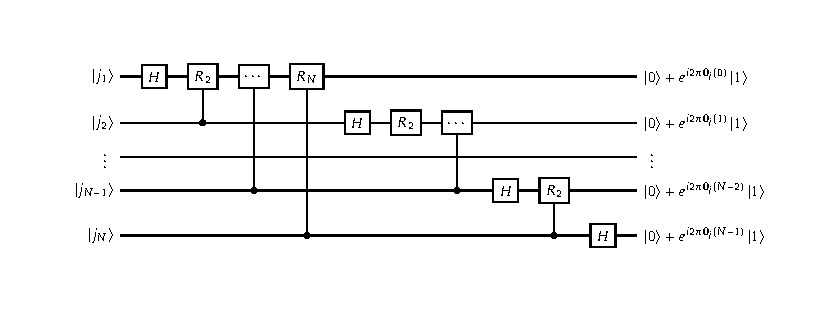
\includegraphics[width=0.9\textwidth]{Immagini/QFT.pdf}
    \caption
    {
        Circuits able to perform the quantum fourier tranform of the computational basis. It's important to notice how this algorithm is in reality not totally complete since the phases of the final states are inverted, so a series of swap gates needs to be inserted at the end to get the right form.
    }
    \label{fig:QFT}
\end{figure}
basically the Hadamart and phase gates. The final form of the circuit is described in \figref{fig:QFT}, where is possible to see how we can evaluate the QFT by the cimple use of controlled phase gates and swaps ones at teh end of the proces. This particular circuit is interesting since shows how quantum computers are able to perform fuorier transforms easily respect to classical algorithm. In fact, the number of gates required to perform such an operation scales as $\mathcal{O}(n^2)$ while the number of logic gates needed to perform the computation of a fast fourier transform inside a classical computer scales as $\mathcal{O}(n2^n)$. Quantum algorithm beats the classical one by an exponential factor. Nevertheless, the quantum algorithm has the big problem that the information are present in the phase of the states, and we are not able to evaluate them, basically meaning that the algorithm alone is useless. Still, we will see that QFT will still be used inside larger algorithm giving a lot of benefits.